\documentclass[a4paper,12pt]{article}

\usepackage[utf8]{inputenc}
\usepackage[T1]{fontenc}
\usepackage[french]{babel}
\usepackage{graphicx}
\graphicspath{{./Images/}}
\usepackage{xcolor}
\usepackage{amsmath, amssymb}
\usepackage[left=3cm,right=3cm,top=2cm,bottom=2cm]{geometry}
\usepackage{listings}

\begin{document}
\begin{figure}
    \centering
    
\includegraphics[width=0.5\textwidth]{enseirb-matmeca.png}
\end{figure}
\begin{center}
\vspace{0.5\baselineskip}
  \Huge
  { \huge \bfseries Acting Shooting Star}\\[0.4cm]
\vspace{\baselineskip}
\large
\begin{center}
 \rule{0.5\linewidth}{1pt}
 \end{center}

Projet réalisé par \\
\large
\vspace{1\baselineskip}
Boullit Mohamed Fayçal\\
Izekki Jalal\\
Moussa Guimba Mamadou\\
Pierre Hugo\\
\begin{center}
 \rule{0.5\linewidth}{1pt}
 \end{center}
\vspace{2\baselineskip}
\large
Projet encadré par \\
\vspace{1\baselineskip}
Calandra Joséphine\\
\large
\vspace{3\baselineskip}
Equipe 9151\\
\vspace{3\baselineskip}
Année 2019/2020
\end{center}


\newpage

\tableofcontents
\newpage

\section{Introduction}

Le sujet de programmation  informatique traité ce semestre est le modèle basé sur les acteurs (\textbf{Actor Model}). C'est un modèle mathématique qui considère un monde remplie d'acteurs qui interagissent entre eux. Dans ce modèle un acteur est une unité fondamentale de calcul; c'est un objet qui reçoit un message et fait une sorte de calcul sur lui même. Tout acteur posséde alors un état propre, envoie mais aussi reçoit des messages d'autres acteurs et met à jour son propre état. \\
Le jeu \textit{Terminal Phase} codé par Christopher Lemmer Webber en langage Racket, est un exemple concret de ce type de programmation.
A l'instar de ce dernier, le but de notre projet est de construire et développer une bibliothéque d'acteurs en Racket menant à l'élaboration d'un jeu qui approche un shoot'em up. 

\section{Structure du Jeu}

Dans l'environnement du jeu se trouvent différents types d'acteurs qui interagissent entre eux en s'envoyant différents types de messages. Pour  une bonne hiérarchisation une horloge de synchronisation découpe le temps en intervalle. A chaque pas de l'horloge, les acteurs reçoivent leurs messages et se mettent à jour en fonction de ce qu'ils ont reçu en attendant le prochain pas de l'horloge.

\subsection{Répresentation des acteurs}
Un acteur est représenté par une structure de données nommée \textbf{Actor} et il est caractérisé par son nom, sa position (x,y) dans l'espace du jeu et sa durée de vie.
Il faut savoir que les messages sont envoyés de manière asynchrone aux acteurs et ces derniers les traitent séquentiellement; d'où la nécessité d'avoir une boîte de messages \textbf{mailbox} où ils peuvent stocker les différents messages.
En outre, les acteurs sont de deux sortes: les vaisseaux et les missiles. Cependant on distingue quatre types d'acteurs à savoir : 
\\

\begin{itemize}

    \item les vaisseaux alliés \textbf{ally-ship}: il existe généralement un seul vaisseau allié, qui est le vaisseau principal. Son objectif est d'attaquer et de détruire les autres vaisseaux \textbf{ennemy-ship}
    \item les vaisseaux ennemis: c'est une masse de vaisseaux qui sort de manière aléatoire du coté ennemis et envahit le vaisseau allié. 
    \item les missiles alliés \textbf{ally-missile}: Ce sont les acteurs créées par le vaisseau allié, qui lorsqu'ils entrent en collision avec les acteurs ennemis les détruisent et meurt également.
    \item les missiles ennemis \textbf{ennemy-missile}: Ceux là sont créées par les vaisseaux ennemis et ont le même rôle que ceux cités précédemment; celui de tuer ou de réduire la durée de vie du vaisseau principal. 
    \\
\end{itemize}

A ceux là s'ajoutent deux autres types d'acteurs:
\\

\begin{itemize}
    \item les acteurs \textbf{obstacle} qui lorsqu'ils rencontrent le vaisseau allié, diminuent sa durée de vie.
    \item les acteurs \textbf{bonus} qui ont pour rôle d'augmenter la durée de vie du vaisseau allié.
\end{itemize}

Ainsi un acteur est représenté de la manière suivante: 

\begin{lstlisting}[language={lisp},captionpos=b, frame=single]
(struct concrete-actor (name location mailbox type health))
\end{lstlisting}

Pour en créer un dans l'espace du jeu, une fonction nommée \textbf{make-actor} qui prend comme paramètre la position et le type de l'acteur, est implémentée. Elle est utilisée par \textbf{(generate-actor tick)} qui crée des acteurs ennemis , obstacles et bonus. A un pas \textbf{tick} donné, elle génère une liste des acteurs avec des ordonnées différentes aléatoires mais avec une même abscisse qui est celle de l'extrémité droite du cadre du jeu; sachant qu'ils se dirigent tous vers l'acteur principal.

\subsection{Représentation et traitement des messages}

Il existe différentes formes de messages en fonction de l'information que l'on souhaite transmettre aux acteurs:
\begin{itemize}
    \item un message \textbf{('move x y)} permet à l'acteur visé de se déplacer de (x, y) dans l'espace du jeu.
    \item un message \textbf{('Collide)} qui peut prendre plusieurs formes. Il dépend des types d'acteurs qui se rencontrent.
    \item un message \textbf{('shoot "-")} qui est envoyé soit au vaisseau principal soit aux vaisseaux ennemis pour pouvoir créer des missiles. 
\end{itemize}

Ces messages sont envoyés à un \textbf{actor} par la fonction \textbf{actor-send} qui retourne alors un nouvel \textbf{actor} contenant le message dans sa \textbf{mailbox}.

Vient alors la fonction \textbf{actor-update} qui met à jour les \textbf{actor} en vidant la \textbf{mailbox}. Pour ce faire, la fonction s'appelle récursivement en modifiant l'\textbf{actor} à l'aide d'autres fonctions appelées en fonction du message.

\begin{lstlisting}[language={lisp},captionpos=b, frame=single]
(actor-send actor message)
(actor-update actor)
\end{lstlisting}

\subsubsection{Move}
Le message \textbf{move} est géré par deux fonctions, la première :
\begin{lstlisting}[language={lisp},captionpos=b, frame=single]
(actor-move actor mvnt)
\end{lstlisting}
prend en paramètre un \textbf{actor} et le mouvement (\textbf{mvnt}) à lui faire réaliser. Ce mouvement est représenté par une liste de deux coordonnées représentant le vecteur du déplacement.

Vient alors l'autre fonction :
\begin{lstlisting}[language={lisp},captionpos=b, frame=single]
(sum-pair-list p l)
\end{lstlisting}
Cette fonction permet de sommer la liste représentant le mouvement et la position de l'\textbf{actor} qui est une \textbf{pair}.

\subsubsection{Collide}
Il y a plusieurs messages pour les collisions chacun correspond à un type de collision entre le vaisseau allié et un autre \textbf{actor}.

Chaque fonction permet une réaction différente en fonction du type de l'\textbf{actor} rencontré et ainsi soit détruire le vaisseau, soit lui réduire sa durée de vie.

\subsubsection{Shoot}
Le message de tire est géré par la fonction \textbf{actor-shoot} qui en fonction du type de l'\textbf{actor} donné en paramètre, créé alors un missile allié ou ennemie à l'avant de l'actor.

\section{Gestion du jeu}

\subsection{Le monde des acteurs}

Pour manipuler le monde des acteurs, une structure \textbf{world} est créée qui regroupe l'ensemble des acteurs dans une liste.
\begin{lstlisting}[language={lisp},captionpos=b, frame=single]
(struct world (actors))
\end{lstlisting}
Cela permet de gérer de manière globale l'ajout des acteurs dans le jeu, les déplacements des acteurs, l'envoi des différents messages mais également la gestion des différentes collisions. \\
\begin{itemize}

    \item[\huge -]L'ajout d'une liste d'acteurs dans le monde se fait à l'aide d'une fonction
    \begin{lstlisting}[language={lisp},captionpos=b, frame=single]
    (world-add-actor world actors)
    \end{lstlisting}
    qui est de complexité en temps linéaire.
    
    \item[\huge -] En ce qui concerne les collisions rappelons qu'un acteur dispose d'une certaine durée de vie qui est constante et négative pour les acteurs ennemis du vaisseau allié mais positive et constante pour ce dernier. 
    Lors d'une collision du vaisseau principal et d'un autre acteur, un message de type \textbf{collide} qui est fonction du type du second acteur, est envoyé aux deux acteurs. Par la suite, à la mis à jour des acteurs le second est détruit et l'acteur principal gagne ou perd en durée de vie.
    Prenons l'exemple d'une collision avec un acteur \textbf{bonus}; dans notre cas nous considérons arbitrairement que ce dernier rapporte 3 unités de plus dans la durée de vie du vaisseau principal, contrairement à une collision avec un missile ennemi qui réduit de 2 unités sa duré de vie. \\
     Ainsi donc, afin de vérifier qu'il y' a des collisions dans le monde des acteurs, une fonction
    \begin{lstlisting}[language={lisp},captionpos=b, frame=single]
    (world-collision world)
    \end{lstlisting}    
    est implémentée. Elle prend récursivement un acteur du world et vérifie d'éventuelles collisions avec le reste des acteurs. S'il y' a collision, elle envoie le message \textbf{collide} aux deux acteurs et passe à un autre acteur, sinon refait la même démarche sur le reste des acteurs. Ce qui donne à cette fonction une complexité quadratique \textbf{$\theta (n^2)$} où n est le nombre d'acteurs dans l'espace de jeu.

    \item[\huge -] L'envoi des différents messages se fait à l'aide d'une fonction:
    \begin{lstlisting}[language={lisp},captionpos=b, frame=single]
    (world-send world msg type)
    \end{lstlisting}
    qui recherche de manière récursif dans world, les acteurs dont le type correspond à celui passé en paramètre et lui envoi le message msg à l'aide de la fonction \textbf{actor-send}. Cette fonction est de complexité en temps linéaire.
    
    \item[\huge -] La mis à jour du monde se fait à l'aide d'une fonction:
    \begin{lstlisting}[language={lisp},captionpos=b, frame=single]
    (world-update world)
    \end{lstlisting}
    qui utilise la fonction \textbf{actor-update} récursivement sur le world mais aussi la fonction \textbf{world-collision} ce qui lui donne d'ailleurs une complexité en temps quadratique.
\end{itemize}
Notons par ailleurs qu'il arrive un moment où certains acteurs sortent du cadre du jeu. Arrivés à l'abscisse 0, ces derniers doivent être détruits vue qu'ils sont arrivés à l'autre extrémité du cadre et qu'ils ne sont plus utiles dans la suite du jeu. La fonction \textbf{(destroy-actor actors)} le fait récursivement sur les différents acteurs. Elle vérifie également que le vaisseau principal se trouve à tout moment dans l'espace du jeu. S'il arrive qu'il sorte du cadre, ce dernier est détruit et le jeu prend fin.


\subsection{Avancement du jeu}
La structure world citée précédemment est placée dans une autre nommée \textbf{runtime} qui contient des messages et l'horloge globale \textbf{tick}. Elle a pour fonction d'envoyer les différents messages aux acteurs du monde \textbf{world} à chaque pas de l'horloge, de les mettre à jour et de renvoyer un nouvel état du monde.

\begin{lstlisting}[language={lisp},captionpos=b, frame=single]
(struct runtime (world messages tick))
\end{lstlisting}

Au début du jeu, le seul acteur présent est le vaisseau principal attendant l'invasion des différents vaisseaux ennemis. A chaque pas de l'horloge \textbf{tick} et avant le prochain pas:
\begin{itemize}
    \item Le runtime ajoute dans son \textbf{world} des nouveaux acteurs, fournis par \textbf{(generate-actor tick)}, à l'aide de la fonction 
    \begin{lstlisting}[language={lisp},captionpos=b, frame=single]
    (runtime-add-actor runtime actors)
    \end{lstlisting}.
    
    \item le runtime par la suite reçoit une liste de messages  par la fonction 
    \begin{lstlisting}[language={lisp},captionpos=b, frame=single]
    (runtime-receive runtime messages)
    \end{lstlisting} avec \textbf{messages} de la forme \textbf{(list (msg type))} où chaque message \textbf{msg} est de type \textbf{move} à envoyer à l'acteur de type \textbf{type}. Cela à pour but de faire avancer d'un pas les différents acteurs.
    
    \item Après avoir reçu ses messages, le runtime vide son champs messages et envoie ces derniers aux différents acteurs à l'aide de la fonction 
    \begin{lstlisting}[language={lisp},captionpos=b, frame=single]
    (runtime-send runtime)
    \end{lstlisting}
    
    \item Enfin le runtime, à l'aide de la fonction
    \begin{lstlisting}[language={lisp},captionpos=b, frame=single]
    (runtime-update runtime)
    \end{lstlisting}, met à jour tout les acteurs et renvoie un nouvel état du monde.
\end{itemize}
Ces étapes sont effectuées successivement à chaque pas de l'horloge globale du jeu.
Toutes les fonctions citées plus haut sont linéaires à l'exception de la fonction de mise à jour qui est quadratique et de la fonction runtime-receive qui est constante.


\subsection{L'interface graphique}


L'affichage des acteurs ainsi que l'interface graphique est faite à l'aide de la bibliothèque \textbf{raart} qui fournie plusieurs fonctions permettant d'afficher du texte sur un terminal.
Pour l'animation du jeu c'est la bibliothéque \textbf{Lux} qui est utilisée. Elle fournit un moyen efficace de créer des programmes interactifs en temps réel. Pour le fonctionnement de la bibliothéque sur notre projet, il s'agit de créer une structure qui représente l'état globale de l'application.
\begin{lstlisting}[language={lisp},captionpos=b, frame=single]
    (struct game (runtime)
    #:methods lux:gen:word)   
\end{lstlisting}
La structure \textbf{game} comprend le runtime ainsi que différentes méthodes qui permettent la gestion de l'état du jeu:
\\

\begin{itemize}
    \item[\huge *] la méthode (word-fps w) renvoie le taux de mise à jour souhaité pour le \textbf{game} en images par seconde.
    
    \item[\huge *] la méthode (word-label w) renvoie le titre de la fenêtre contenant le jeu.
    
    \item[\huge *] la méthode (word-event w e) qui à partir d'un état du monde et d'un évènement \textbf{e} renvoie un nouvel état du monde. C'est cette méthode qui permet l'interaction entre le jeu et l'utilisateur.C'est ainsi que pour faire déplacer le vaisseau principal, l'utilisateur tape sur les touches de direction de son clavier et cette fonction envoie un message move ou shoot à l'acteur principal en fonction de la touche enfoncé sur le clavier. Rappelons par contre que seul le vaisseau principal est manipulable par l'utilisateur; le reste des acteurs est gérer par le runtime.
    
    \item[\huge *] la méthode (word-output w) qui permet d'afficher n'importe quel objet graphique.
    
    \item[\huge *] la méthode (word-tick w) qui permet la mise à jour des différents acteurs et renvoie un nouveau monde.
    
    \item[\huge *] la méthode (word-return w) qui affiche un message en cas d'éventuelles erreurs.
  \\  
\end{itemize}

\begin{figure}[h]
    \centering
    \label{fig:actor}
    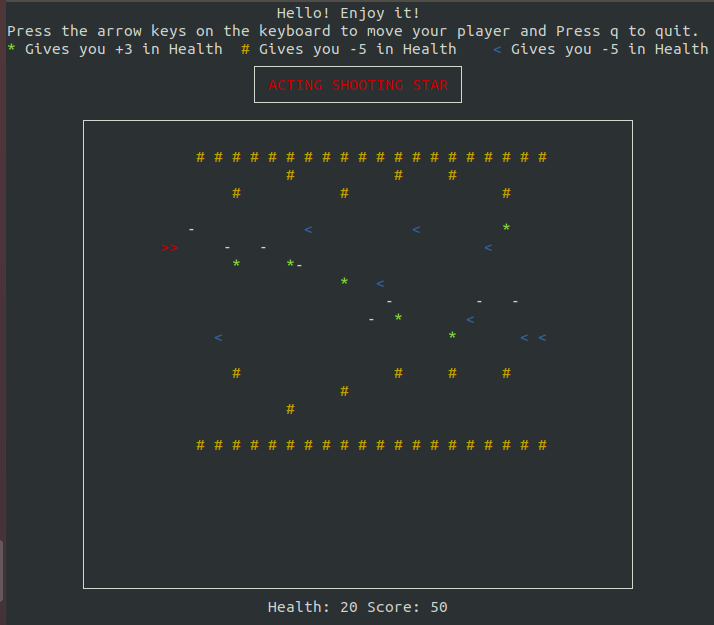
\includegraphics[width=0.9\textwidth]{Images/actor.png}
    \caption{L'interface graphique du jeu}
\end{figure}

A partir de la figure 1 nous pouvons visualiser la manière dont sont représentés nos différents acteurs:
\\

\begin{itemize}
    \item \textcolor{red}{\huge >>} représente l'acteur principal,
    \item \textcolor{blue}{\large <} représente un vaisseau ennemi et fait perdre 2 unités de vie au vaisseau principal,
    \item \textcolor{gray}{\huge -} représente un missile et fait perdre également 2 unités de vie au vaisseau principal,
    \item \textcolor{orange}{\#} représente un acteur obstacle. Il fait perdre 5 unité de vie au vaisseau principal,
    \item \textcolor{green}{\large *} représente un bonus et fait gagner 3 unités de vie au vaisseau principal
\end{itemize}




\section{Tests et documentation du projet}
\subsection{Les tests}
Les tests pour ce projet ont été réalisés à l'aide de la bibliothèque \texttt{rackunit}. Il sont décomposés en 3 fichiers. Chaque fichier contient une \texttt{test-suite}:
\begin{itemize}
    \item Un fichier \texttt{test-actor.rkt}: teste les fonctions du fichier \texttt{actor.rkt}. Les fonctions testées sont \texttt{actor-location}, \texttt{actor-send} et \texttt{actor-update}.
    \item Un fichier \texttt{test-world.rkt} pour tester les fonctions \texttt{world-send}, \texttt{actors-collision} et \texttt{world-update} du fichier \texttt{world.rkt}.
    \item Un dernier fichier \texttt{test-runtime.rkt} pour tester les deux fonctions \texttt{runtime-send} et \texttt{runtime-update}.
\end{itemize}
La commande \texttt{make test} permet d'exécuter l'ensemble de ces fichiers et afficher les résultats des tests.
\subsection{Documentation}

La documentation de ce projet est réalisée avec \textbf{Scribble} qui est un outil de description ressemblant au langage \LaTeX. Les fichiers écrits avec cet outil  en plus du fichier principal \texttt{doc.scrbl} sont les suivants:
\begin{itemize}
    \item Un fichier \texttt{actor.scrbl} pour décrire le code du fichier \texttt{actor.rkt}.
    \item Un fichier \texttt{world.scrbl} contenant la documentation des fonctions et structures de \texttt{world.rkt}.
    \item Un fichier \texttt{runtime.scrbl} qui montre le fonctionnement du code de \texttt{runtime.rkt}.
\end{itemize}
La commande pour générer la documentation est \texttt{make doc}.
Cette commande permet de générer plusieurs fichiers et les mettre dans le répertoire \texttt{doc}. Pour visualiser la documentation, il suffit d'ouvrir le fichier \texttt{doc.html}.

\section{Conclusion}

\subsection{Perspective et suite du projet}
Ce projet nous a permis de développer un jeu du style shoot'em up, dans lequel le joueur joue un vaisseau qui se défend d'une invasion ennemie, toute fois nous n'avons implémenté qu'un seul niveau de difficulté. Dans la continuité, nous pourrions donc implémenter différents niveaux de difficultés comme par exemple des vaisseaux ennemies qui tire des missiles, en augmenter le nombre ou bien des vaisseaux ennemis qui lorsqu'ils sont détruits en libèrent d'autres.

\subsection{Les apports du projet}
Ce projet nous a permis de réaliser un projet en Racket qui est un langage fonctionnel or les autres projets que nous avions réalisé étaient dans des langages impératifs, or la programmation fonctionnelle est une autre façon de voir la programmation.

De plus, ce projet nous à également permis de découvrir les modules racket \textbf{raart} et \textbf{lux}.



\end{document}
